\documentclass[oneside,openright,frontopenright]{dmathesis}
\input{preamble}
\bibliography{bibliography}

\begin{document}
\title{Null geodesics}
\subtitle{Modelling light in the Schwartzschild metric}
\author{Joseph A Sweeney}
\researchgroup{Mathematics}
\pagenumbering{roman}
\maketitlepage*

\begin{abstract}
%
	In this paper I will show and discuss my findings on numerical methods and optimisations for modelling solutions to the geodesic equations generated by a Schwarzschild metric using Python. In the first section, I will introduce some key information and language associated with General Relativity, which this paper will rely on. Then, I will show multiple methods for modelling a null (light-like) geodesic about a Schwarzschild black hole. Finally, I will walk through a method for modelling a pinhole camera a fixed distance away from a Schwarzschild black hole, with any given celestial sphere.
%
\end{abstract}

\begin{declaration*}
%
	The work in this thesis is based on research carried out in the Department of
	Mathematical Sciences at Durham University. No part of this thesis has been
	submitted elsewhere for any degree or qualification.
%
\end{declaration*}

\disableprotrusion
\tableofcontents*
\enableprotrusion

\cleardoublepage
\pagenumbering{arabic}

%\include{background}
%\include{paper1}
%\include{paper2}
%\include{paper3}
\begin{introduction}

	The field of black hole imaging in Physics and Computer Science had a wave of enthusiasm 
	and development following Christopher Nolan’s 2014 blockbuster Interstellar[1], and the imaging of the supermassive 
	black hole at the centre of M87 by the Event Horizon Telescope in 2019[2]. Producing high quality images 
	and videos of black holes and wormholes can be very computationally costly, so ingenious ways of gaining 
	efficacy must often be used. My aim is to explore these methods and tricks to present practical approaches 
	to modelling various spacetime metrics, including the Schwarzschild metric, Kerr metric, and the Ellis wormhole.

\end{introduction}

\chapter{Introduction to General Relativity}
	Albert Einstein’s theory of General Relativity is a pivotal achievement in the scientific community, here, I will attempt to briefly summarise some key components and notation for ease of readers in later sections.

	In his theory of General Relativity, Einstein formalised gravity not as a force, as it is thought of in Newtonian physics, but as the curvature of spacetime. Spacetime is the 4-dimentional plane we exist in, one dimension from time, and three from space. The path of an object acted upon solely by gravity can be thought of as moving along curved spacetime, with the path being a straight line if the effects of gravity are none-existent. Such a path through curved spacetime is called a geodesic, and equations of motion in General Relativity are governed by constants derived from geodesic equations – which in turn are derived from the metric in which the object finds itself. A null-geodesic, or light-like geodesic, is a path describing the motion of a massless object: In this paper, a null-geodesic will always be describing the path of a light particle in a metric.

	As is common in papers studying light and the astrological, I will be using natural units: That is, I will be taking c = G = 1, this results in sizes of units being shifted, but since we don't calculate distances directly this should not affect us.

	Metrics are sections of spacetime which are solutions to Einstein’s field equations, the equations that define his General theory, for example, the simplest solution to these field equations describing a black hole is the Schwarzschild metric. The relation between geodesic equations and metrics are Christoffel symbols, denoted $\Gamma$, seen in the below general form of a geodesic equation [3]:  


	${\frac{d^2 \gamma^\lambda}{dt^2} + {\Gamma^\lambda}_{\mu\nu} \frac{d\gamma^\mu}{dt} \frac{d\gamma^\nu}{dt} = 0}$

\chapter{Solving general relativistic equations of motion}
\section{Deriving the equations of motion}
	Equipped with equations of motion derived from the geodesic equation determined by the metric we are given; we can solve these equations numerically to visualise the path of light in such a metric. We will start with the Schwarzschild metric, given in line notation by[4]: 


	${ds^{2} = {(1-\frac {2m}{r})}^{-1}} {dr^2} + {r^2}({d\theta ^2} + {\sin ^2}{\theta}{d\varphi ^2}) -{(1-\frac {2m}{r})}{dt^2}$


	Since the metric is spherically symmetric, we see that every path will always be contained in a plane intersecting the origin of the black hole. Therefore, without loss of generality we can take ${\theta}=\frac{\pi}{2}$ and just look ‘from above’ the equatorial plane to see the path of such a light ray in the plane.

	From the above equation, one can derive the equations of motion of a null geodesic in the Schwarzschild metric:


	$\ddot{r}=-\frac{L^2(3M-r)}{r^4}$

	$\dot{\theta}=\frac{L}{r^2}$


	Where M is the mass of the black hole, L is a constant proportional to the angular momentum of the light ray, r is the distance from the centre of the black hole, and $\varphi$ is the angle from the positive x axis to the light ray.

\section{Methods for solving the system}
	The simplest method of solving such an equation numerically is to split the equation into a coupled first order differential equation, and then keep track of r and $\varphi$. Then use your favourite numerical approximation to update for each point in a time array, if you keep track of r and $\varphi$ for all points in the time array you can then plot the path. One thing to be careful about is that as soon as light is within r = 2M, solutions will not make any sense, so do not have an initial position in this region, and ideally while keeping track of r, cut the process off when r = 2M.

	This method is both the simplest and most effective for solving second order ODE’s numerically, the only difference between a ‘bad’ and ‘good’ method would be your choice of numerical approximation method to solve the first order ODE’s

\begin{figure}
	\centering
	\begin{minipage}[b]{0.6\textwidth}
		\includegraphics[width=\textwidth]{img/points200byhand}
		\caption{A plot with 200 points in the time array using short distances to approximate the slope of the line and continue in that direction}
	\end{minipage}
	\hfill
	\begin{minipage}[b]{0.6\textwidth}
		\includegraphics[width=\textwidth]{img/points200scipy}
		\caption{A plot with 200 points in the time array using scipy.integrate.odeint[5]}
	\end{minipage}
\end{figure}


	I have found that for a plot of the path of a photon (Figure 1), the ideal method is scipy.integrate.solve\_ivp, using LSODA \cite{hindmarsh2005lsoda}, this is as the Explicit Runge-Kutta method of order 5 (RK45) \cite{fehlberg1969low}, the inherent method of solve\_ivp is very efficient but not smooth, so makes for unattractive plots. Later, when all we need is to solve, I will be using RK45. Also, solve\_ivp allows one to keep track of an ‘event’, and return if the event took place, moreover one may choose to cut off the calculation process when the event takes place. Naturally this is very useful in our case, as all we need to set the event to is r < 2M.


\chapter{Imaging a black hole}
\section{Outline of the method}

	We now have the means to start thinking about how to model a black hole of distance r away from a camera, with any given celestial sphere. The celestial sphere from a point in space is an image of all the points taken to be arbitrarily far away - for earth it is the sky excluding the moon, mercury and mars. (My 'arbitrary distance' is t=1000 i.e the distance light travels in a vaccum in 1000 seconds)

	Our method for imaging a Schwarzschild black hole will be to first find the minimum angle one may fire a photon from the camera without the photon being absorbed by the singularity. Then, for all angles between this minimum angle and just under $\frac{\pi}{2}$, we will find a relation between angle fired and final angle after t=1000.

	We will then conceptualise a pinhole camera, with its focal point the position of our camera which fires light, some distance r from the centre of the black hole. Using the relation outlined above, we can take any given line of pixels which passes through the centre of the image we take as out celesial sphere, and see where each pixel should end up. Then, by 'rotating' the pinhole camera - or by rotating this central line, we may find where each pixel in our new picture draws its light from on the celestial sphere.

\section{Finding $\alpha_{min}$}
	
	The method used in this section is based on [8, p.2]: To find the minimum angle at which a light ray escapes the gravitational pull of the black hole, I send out a number of angles ranging from 0 to $\frac{\pi}{2}$, then, as soon as an angle does not lead to a termination of solve\_ivp, I repeat this process with much smaller intervals between the previous and current angle. This leads to an accurate $\alpha_{min}$.

\section{The relationship between $\alpha$ and $\alpha^{'}$}

	Here, $\alpha$ is the angle at which the light ray is fired at, and $\alpha^{'}$ is the angle from the camera to the final position of the light ray (See Figure 3.2).
\begin{figure}
	\centering
	\begin{minipage}[b]{0.6\textwidth}
		\includegraphics[width=\textwidth]{img/alpha_alpha-prime}
		\caption{A plot with $\alpha$ = 0.5, $\alpha^{'}$ = 0.242 at an initial distance of 100 along the equatorial plane (t = [0,200], r(0) = 100, $\dot{r}$(0) = -1, $\varphi$(0) = -$\pi$, M = 4, )}
	\end{minipage}
\end{figure}

	By running this program across angles from $\alpha_{min}$ to 1.5 and plotting $\alpha$ on the x-axis with $\alpha^{'}$ on the y axis we find the relationship between $\alpha$ and $\alpha^{'}$. For $\alpha$ between -1.5 and -$\alpha_{min}$ we may take -f(-$\alpha$), where f is the function relating the two. Here we have covered -1.5 to 1.5 radii, nigh on a full field of view.

	When $\alpha \approx \alpha_{min}$ or $-\alpha \approx -\alpha_{min}$ the light ray might semi-orbit or even fully orbit the black hole, meaning I had to be careful in my method  of calculating $\alpha^{'}$. To avoid errors I kept track of the change in $\varphi$, the angle from the current position of the ray to the centre of the black hole. When taking this value modulo $2\pi$, I could see how many orbits the ray had undergone. The main issue with not doing this is for a plot of the function 4, in application we want the angle $-\pi<\alpha^{'}<\pi$.

\begin{figure}
	\centering
	\begin{minipage}[b]{0.6\textwidth}
		\includegraphics[width=\textwidth]{img/alpha-prime_f(alpha)}
		\caption{A plot of the function f, relating $\alpha$ to $\alpha^{'}$ (t = [0,1000], r(0) = 100, $\dot{r}$(0) = -1, $\varphi$(0) = -$\pi$, M = 4)}
	\end{minipage}
\end{figure}

\section{Modelling the black hole}
	
	As outlined in 3.1, here we will give our code a star field to treat as a celestial sphere, and see how a black hole affects the image. To do this, the first thing I do is to calculate the distance in pixels from the middle of the picture to a corner, this will be our 1.5 radians. Then, for every pixel on the original image I calculate the angle $\alpha$ implied by the distance from the pixel to the centre of the image. Then, we use an interpolation technique on our relationship between $\alpha$ and $\alpha^{'}$ to calculate the angle along the straight line intersecting the current pixel and the central pixel at which the light ray would end. Then by converting this angle back to distance we update a copy of the picture to switch the current pixel for the closest pixel to the end point on the original picture.

\begin{figure}
	\centering
	\begin{minipage}[b]{0.6\textwidth}
		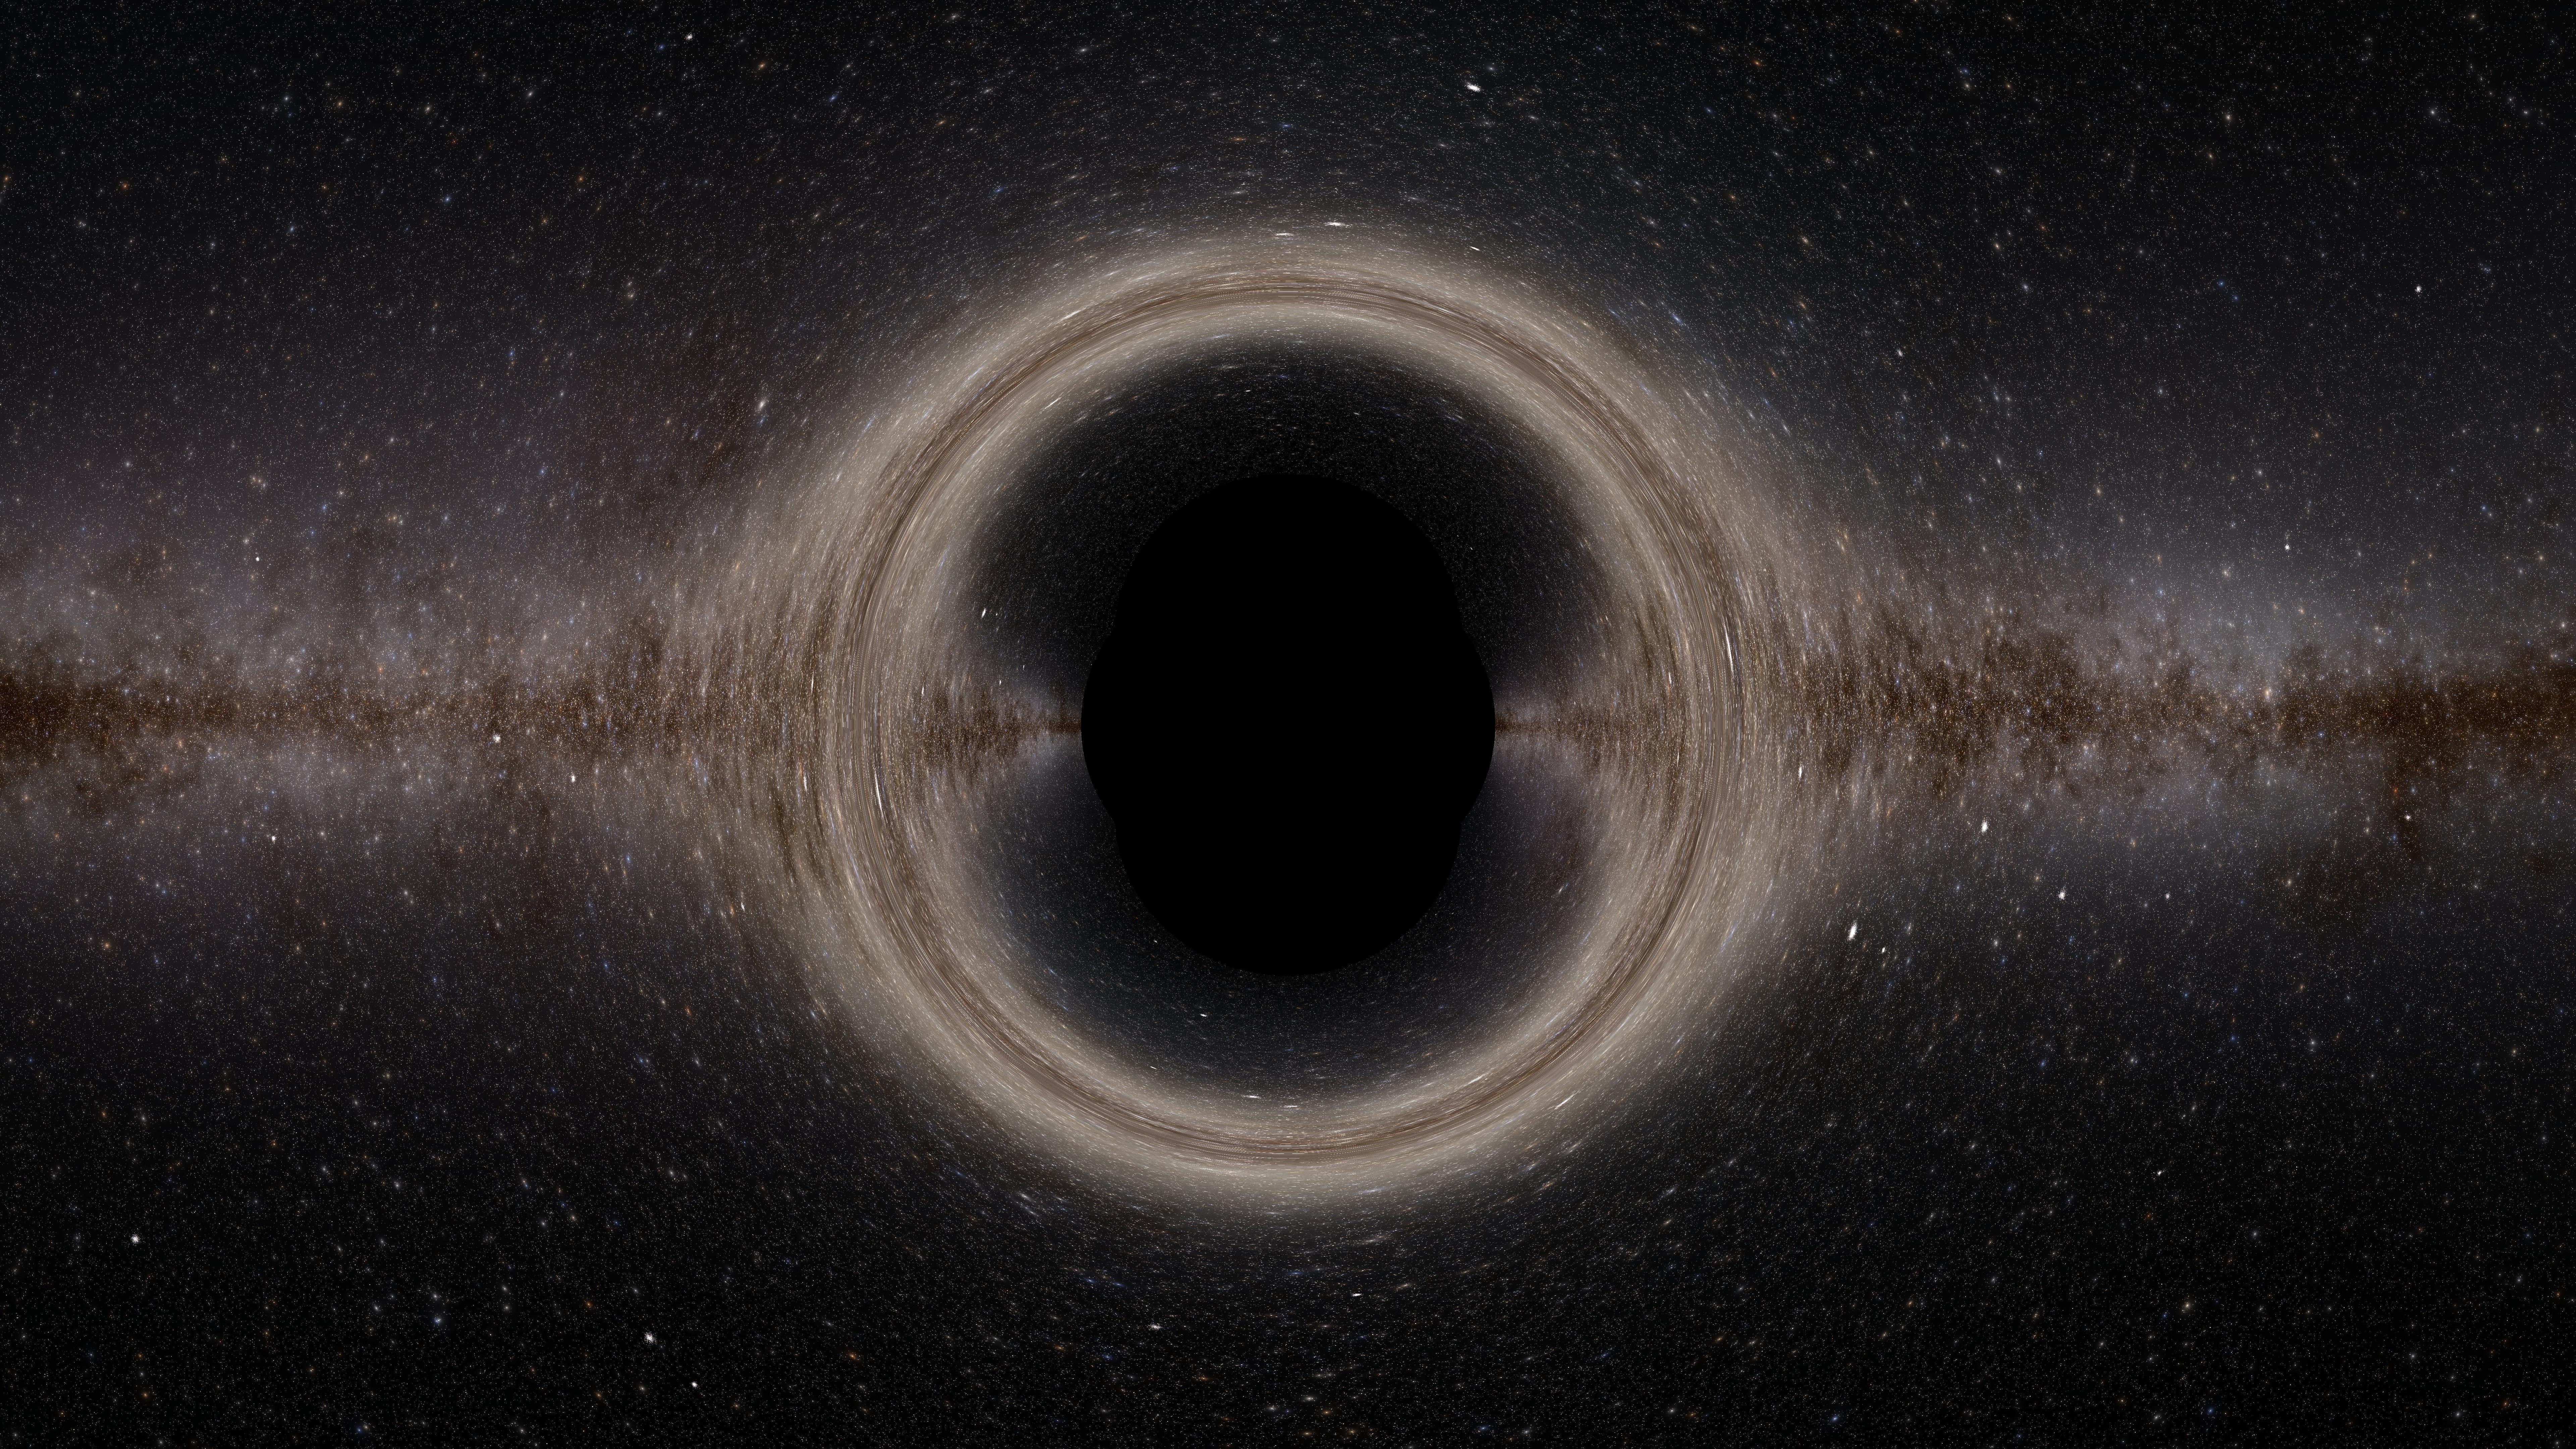
\includegraphics[width=\textwidth]{img/high_quality}
		\caption{A model of a camera with the milkyway as its celestial sphere, with a Schwarzschild black hole directly in front of it}
	\end{minipage}
	\hfill
	\begin{minipage}[b]{0.6\textwidth}
		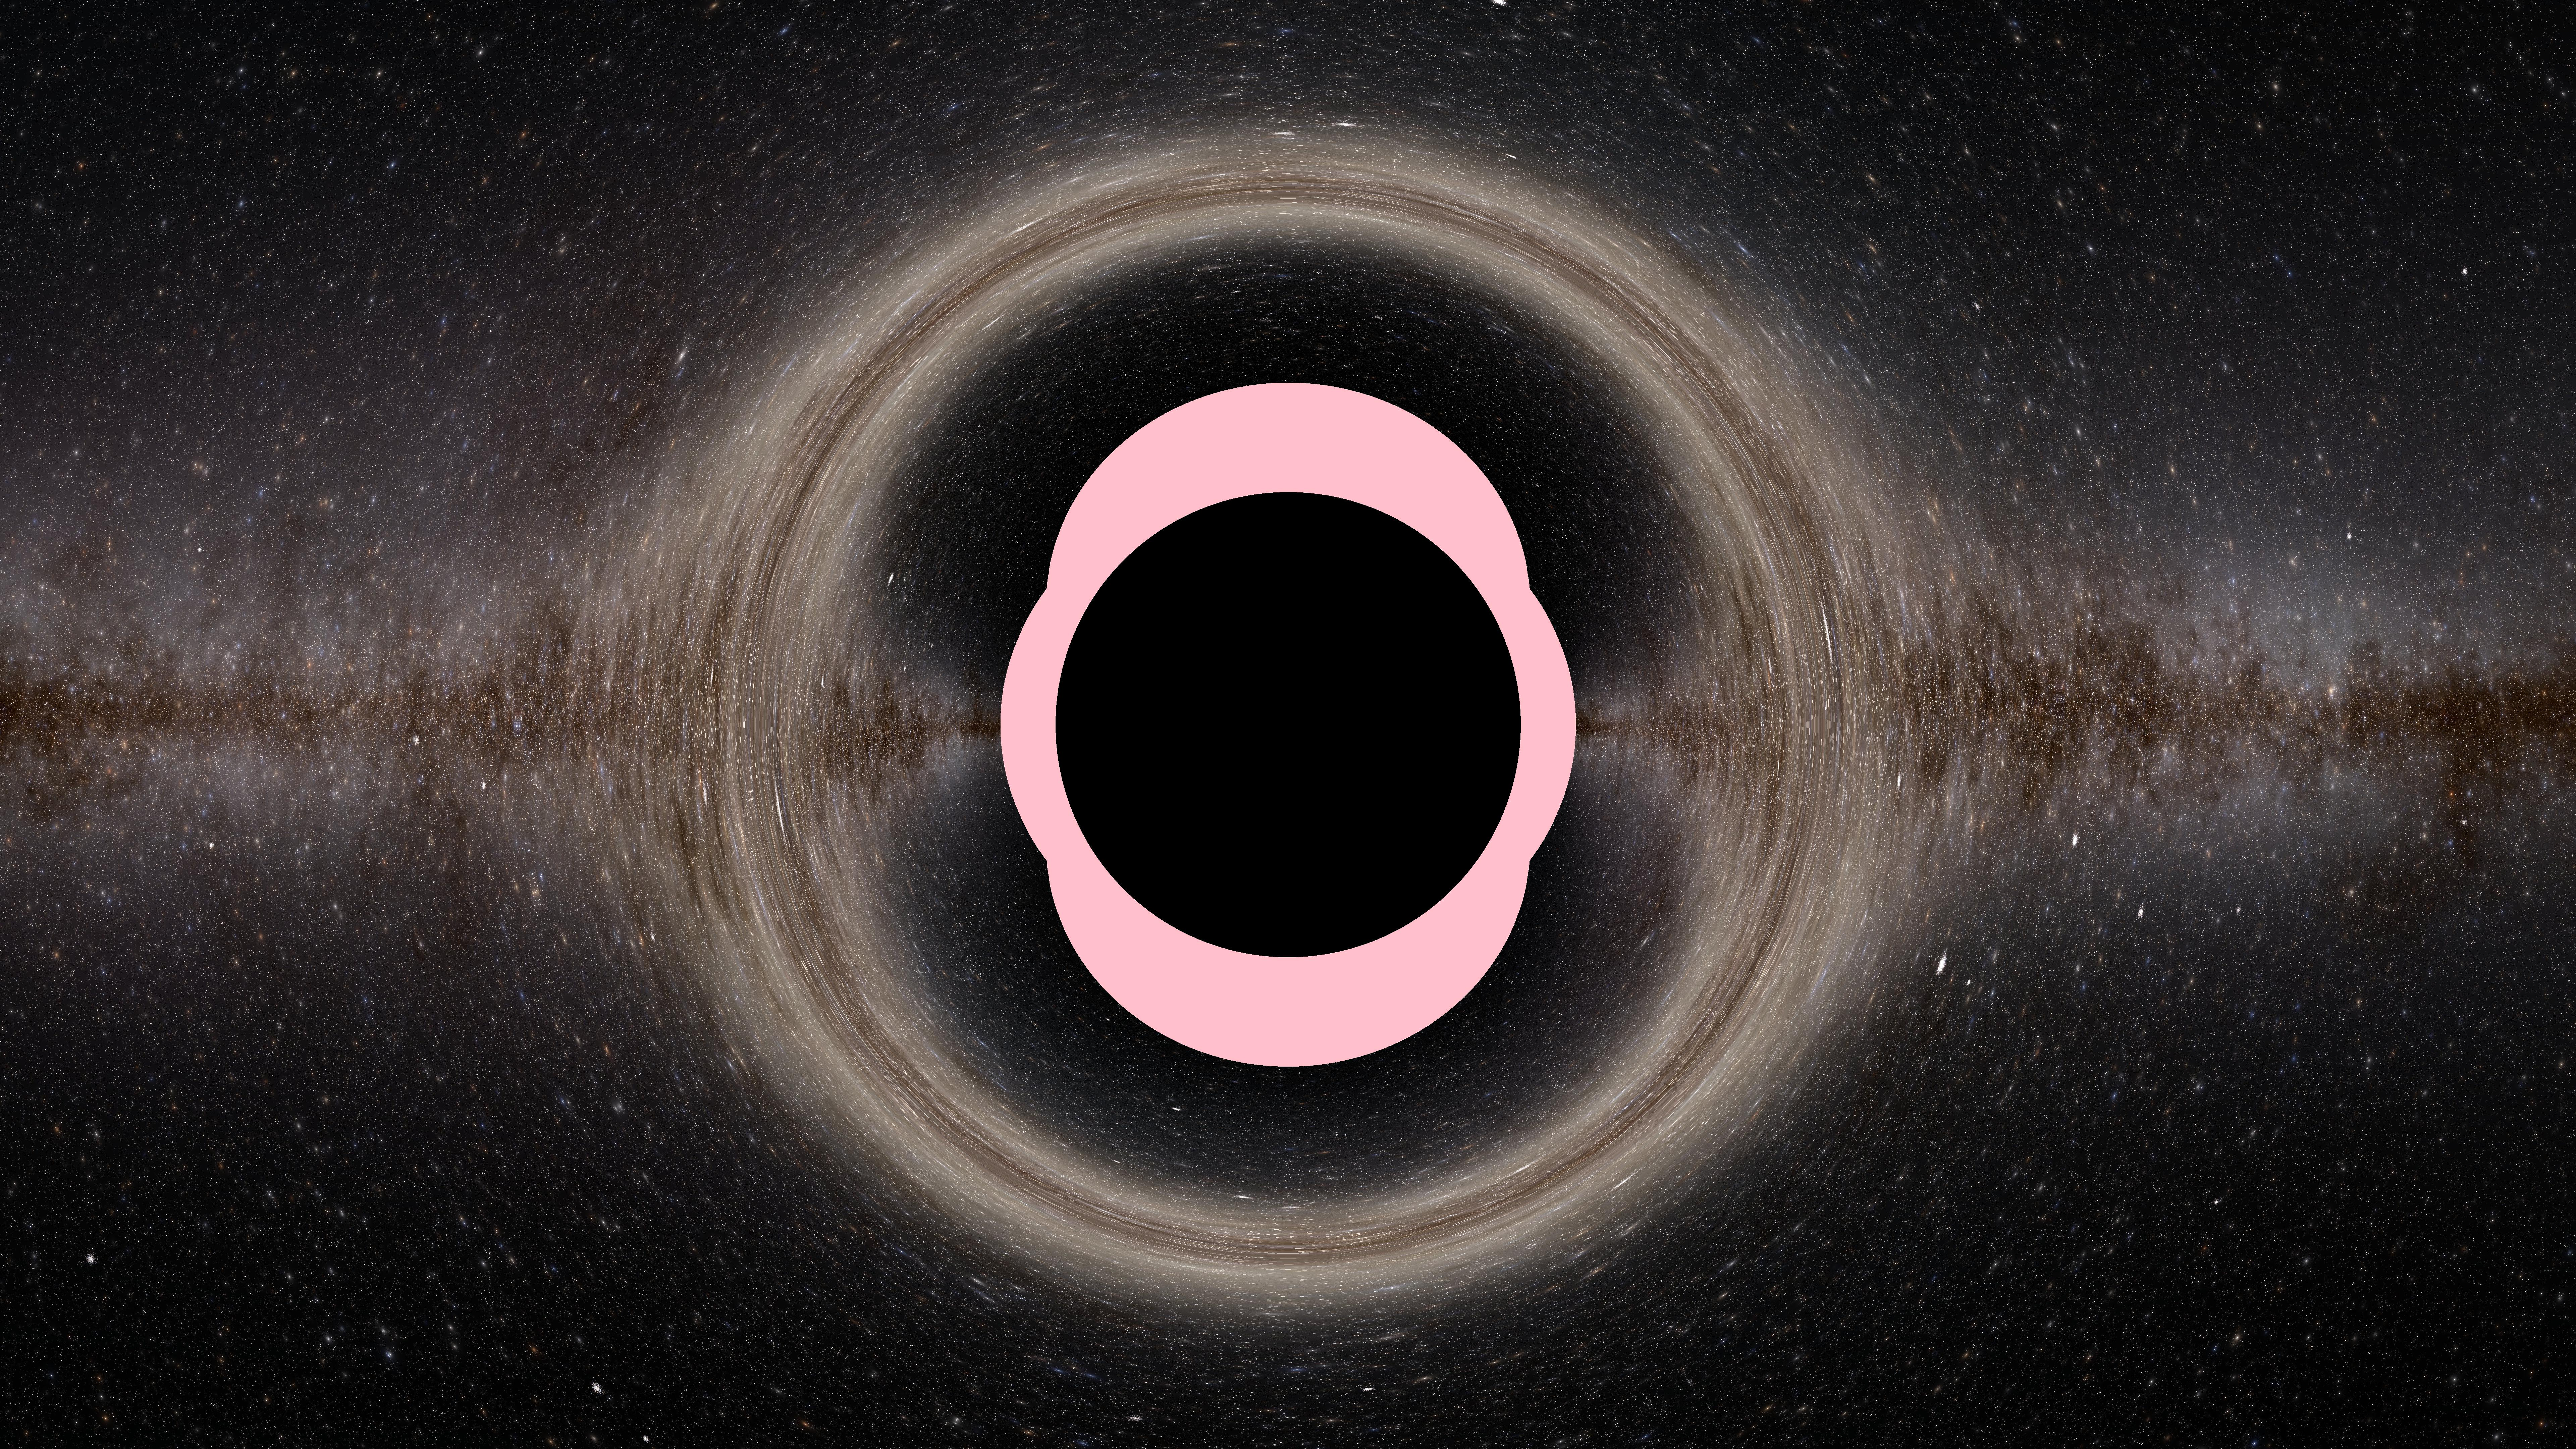
\includegraphics[width=\textwidth]{img/8kstarfield-special}
		\caption{A model highlighting areas affected by the limited size of the image.}
	\end{minipage}
\hfill
	\begin{minipage}[b]{0.6\textwidth}
		\includegraphics[width=\textwidth]{img/hdri}
		\caption{A model using a HDRI image for the celestial sphere.}
	\end{minipage}
\end{figure}

	One issue with this currently is that I am not using an image covering $4\pi$ steradians[9], meaning any ray which leaves the area covered by the original image will lead to a black pixel. This leads to an irregularly shaped black hole (See Figure 3.4), if the image I used as a celestial sphere were circular, the black hole would seemingly look ordinary, as the irregularities would be smoothed out horizontally and vertically, but would be too large. My solution to this was to use a HDRI image and look at 3.1 radii field of view for both the x and y axis (See figure 3.5).

\appendix
%\include{appendix1}
%\include{appendix2}

\nocite{}
\printbibliography[heading=bibintoc]

\end{document}